\chapter{TINJAUAN PUSTAKA}
\label{chap:tinjauanpustaka}

% Ubah bagian-bagian berikut dengan isi dari tinjauan pustaka

Demi mendukung penelitian ini, dibutuhkan beberapa teori penunjang sebagai bahan acuan dan referensi. Dengan demikian penelitian ini menjadi lebih terarah.

%------------------------------------------
\iffalse

% Contoh input gambar
\begin{figure}[ht]
  \centering

  % Ubah dengan nama file gambar dan ukuran yang akan digunakan
  \includegraphics[scale=0.35]{gambar/roketluarangkasa.jpg}

  % Ubah dengan keterangan gambar yang diinginkan
  \caption{Peluncuran roket luar angkasa \emph{Discovery} \citep{roketluarangkasa}.}
  \label{fig:roketluarangkasa}
\end{figure}
\% Contoh pembuatan persamaan
\begin{equation}
  \label{eq:hukumpertamanewton}
  \sum \mathbf{F} = 0\; \Leftrightarrow\; \frac{\mathrm{d} \mathbf{v} }{\mathrm{d}t} = 0.
\end{equation}
\fi
%------------------------------------------

\section{Dasar Teori}
\label{sec:dasarteori}

\subsection{Autonomous Vehicle}

\textit{Autonomous Vehicle} atau kendaraan otonom dapat didefinisikan sebagai kendaraan yang mampu melihat lingkungannya, memutuskan rute apa yang akan digunakan untuk mencapai tujuannya, dan mengendarai dirinya secara mandiri. Dengan kata lain bisa dikatakan kendaraan otonom adalah kendaraan pintar atau robot yang menggunakan berbagai sensor, prosesor komputer, dan basis data untuk mengambil alih beberapa atau semua fungsi mengemudi dari operator manusia. Mobil yang dilengkapi teknologi ini akan memiliki kelebihan tersendiri seperti mengurangi tabrakan, energi konsumsi, dan juga polusi.\cite{cit:autonomous_vehicle_future}

\textit{Society of Automotive Engineers }(SAE) \textit{International }mengeluarkan standar dalam tingkatan dari kemudi	otomatis. Terdapat enam tingkatan dalam standar tersebut. Tingkatan – tingkatan tersebut yaitu:\cite{cit:sae_def}
\begin{figure}[H] 
	\centering
	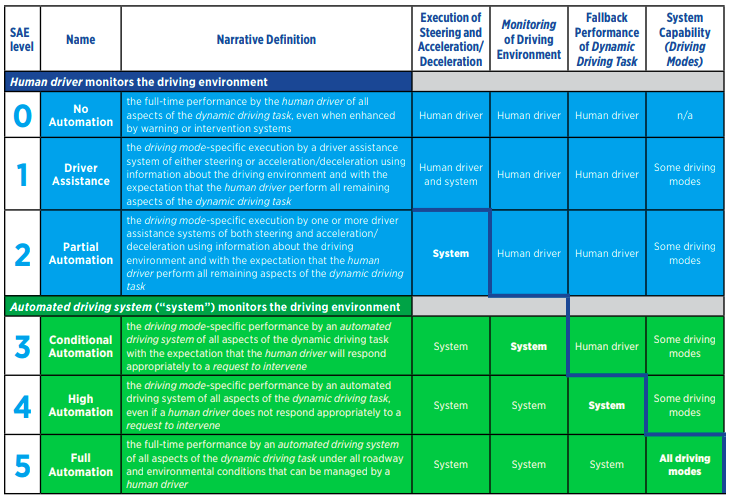
\includegraphics[width=.7\linewidth]{images/autonomous_vehicle_level}
	\caption{Level dari \textit{Autonomous Vehicle }}
	\label{fig:autonomous_vehicle_level}
\end{figure}

\begin{enumerate}[leftmargin=2\parindent]
	\item Level 0, tanpa otomasi. Semua	aspek tugas mengemudi diberikan pada manusia, bahkan ketika ditingkatkan dengan sistem peringatan atau intervensi
	\item Level 1, pendampingan kemudi. Pada tingkat ini fitur-fitur otomasi mulai diterapkan untuk mendukung aspek keselamatan, keamanan, dan kenyamanan pengemudi selama berkendara.
	\iffalse
	\item Level 1, pendampingan kemudi. Adanya bantuan kemudi tertentu oleh sistem kemudi seperti sistem setir atau percepatan/perlambatan dengan menggunakan informasi lingkungan sekitar. Pengemudi manusia melakukan aspek tugas mengemudi yang tersisa.
	\fi
	\item Level 2, otomasi parsial. Kendaraan memiliki minimal 2 fitur otomatis seperti \textit{Steering }dan \textit{Lane Control Assistant }serta \textit{Traffic Jam Assistant}. Sistem mengerem secara otomatis, akselerasi otomatis, dan perlahan–lahan mengambil alih sistem kendali.
	\item Level 3, otomasi kondisional.Kendaraan otonomous level 3 mampu mengemudi sendiri, tetapi hanya dalam kondisi ideal dan dengan keterbatasan. Seorang Pengemudi manusia masih harus mengambil alih jika kondisi jalan berada di bawah kondisi ideal.
	\item Level 4, otomasi tinggi. Kendaraan otonom level 4 dapat mengemudi sendiri tanpa interaksi manusia tetapi akan dibatasi untuk kasus penggunaan yang diketahui. Fitur autonomous Kendaraan level 4 masih dapat dioperasikan hanya pada lingkungan tertentu. 
	\item Level 5, otomasi penuh. Kendaraan berkemampuan level 5 harus dapat memonitor dan bermanuver melalui semua kondisi jalan dan tidak memerlukan intervensi manusia apa pun, menghilangkan kebutuhan akan roda kemudi dan pedal.
\end{enumerate}

Saat ini, level otomasi SAE dari iCar ITS berada pada antara level 3 sampai level 4. \cite{cit:icar_its_news}

\subsection{Machine Learning}

\textit{Machine learning} adalah sebuah cabang dari \textit{artificial intellegence} (AI). \textit{artificial intellegence} memiliki pengertian yang sangat luas, umumnya memiliki arti bagaimana komputer bisa memiliki kecerdasan seperti halnya manusia. \textit{Machine Learning }menurut Arthur Samuel, seorang ilmuwan di bidang komputer yang mencetuskan kecerdasan buatan (\textit{artificial intellegence}) pertama kali, adalah sebuah bidang yang memberi kemampuan komputer untuk belajar tanpa diberi program secara eksplisit. \textit{Machine learning} menggunaan metode statistika untuk membuat komputer dapat mempelajari pola pada data atau biasanya disebut sebagai \textit{pattern recognition}. \cite{cit:ml_patternrecog}

\subsection{Deep Learning}
\begin{figure}[H] 
	\centering
	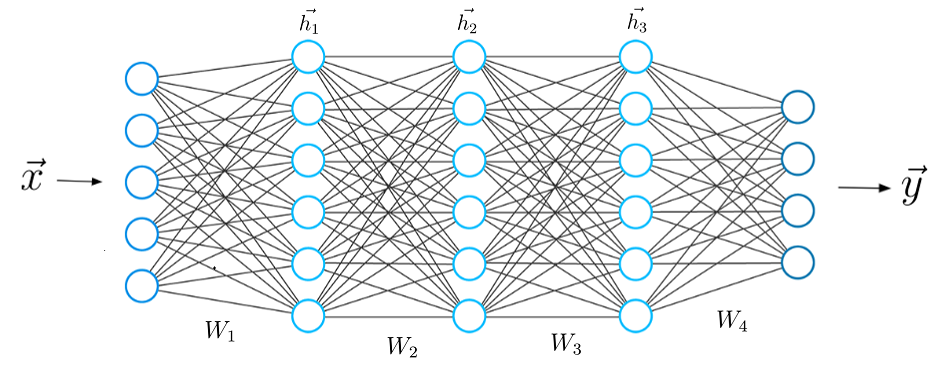
\includegraphics[width=.4\linewidth]{images/deep_learning}
	\caption{Deep Learning}
	\label{fig:deep_learning}
\end{figure}
\textit{Deep learning} merupakan salah satu bagian dari \textit{machine learning}. \textit{Deep learning} dapat dikatakan sebagai algoritma yang menggunakan jaringan syaraf tiruan (\textit{Artificial Neural Network} atau disingkat ANN) untuk menyelesaikan permasalahan pada domain \textit{machine learning}. ANN digunakan sebagai pendekatan dalam pengolahan informasi yang terinspirasi dari bagaimana tiap neuron dalam otak manusia bekerja. Tiap saling berhubungan dan informasi mengalir dari suatu neuron ke neuron lainnya. \cite{cit:deep_learning}

\subsection{Reinforcement Learning}
\begin{figure}[H] 
	\centering
	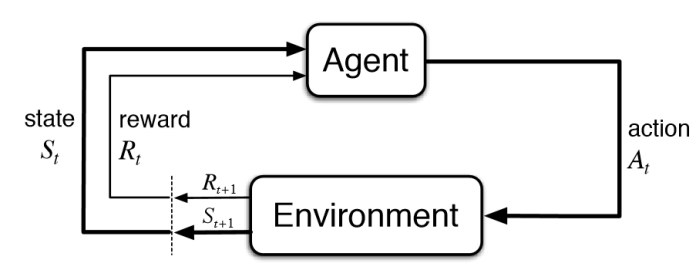
\includegraphics[width=.4\linewidth]{images/reinforcement_learning}
	\caption{Reinforcement Learning}
	\label{fig:reinforcement_learning}
\end{figure}
\textit{Reinforcement Learning }adalah salah satu teknik dari \textit{Machine Learning }dimana \textit{agent }belajar berdasarkan pengalaman yang dialami oleh \textit{agent }tersebut dengan dilengkapi sedikit atau tanpa pengetahuan sebelumnya. \textit{Reinforcement Learning }mempelajari sesuatu hal dengan cara melakukan aksi tertentu dan melihat hasil dari aksi tersebut.\cite{cit:rl_book}

\subsubsection{Skema Kerja Reinforcement Learning}
Seperti pada Gambar \ref{fig:reinforcement_learning}, agen (agent) menerima informasi dari lingkungan (environment) dalam bentuk state. Agen merupakan subjek utama yang melakukan pembelajaran. Lalu, agen memutuskan action apa yang perlu dilakukan berdasarkan informasi lingkungan yang telah didapatkan. Action merupakan serangkaian kemungkinan gerakan yang akan dilakukan oleh agen. Setelah action dilakukan, lingkungan akan berubah dan memberi informasi state baru disertai dengan reward yang didapatkan.

Reward adalah skor yang dapat bernilai positif atau negatif sesuai dengan informasi yang didapatkan dari lingkungan. Agen akan belajar dan melakukan transisi dari state awal hingga state akhir. Proses pembelajaran dari awal hingga akhir ini disebut dengan episode. Sementara state, reward, dan action di tiap perjalanannya dikenal dengan istilah trajectory. Tujuan dari agen adalah untuk memaksimalkan reward yang diperoleh dengan memilih action yang tepat dalam tiap state-nya. Perilaku agen dalam menentukan action yang dipilih berdasarkan state yang diperoleh disebut dengan policy

Salah satu permasalahan yang dihadapi dalam reinforcement learning adalah memodelkan lingkungan yang tepat dalam melakukan pembelajaran terhadap agen. Karena dibutuhkan banyak percobaan yang berulang-ulang untuk dapat memperoleh hasil pembelajaran yang baik, maka perlu dilakukan pembelajaran di Simulator yang tepat sebelum algoritma dapat diimplementasikan di lingkungan sebenarnya.
\iffalse
\subsubsection{Markov Decision Process (MDP)}
\subsubsection{Value Function}
\fi
\subsection{Deep Reinforcement Learning}
\begin{figure}[H] 
	\centering
	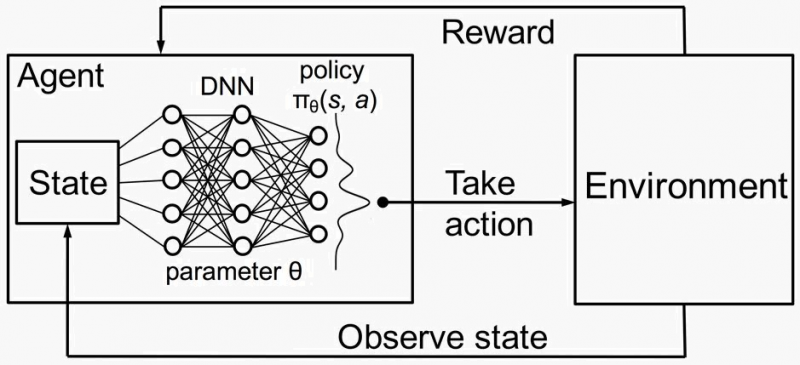
\includegraphics[width=.4\linewidth]{images/deep_rl}
	\caption{Deep Reinforcement Learning}
	\label{fig:deep_reinforcement_learning}
\end{figure}
\textit{Deep Reinforcement Learning }(deep RL) adalah subbidang \textit{machine learning }yang menggabungkan \textit{reinforcement learning }(RL) dan \textit{deep learning}. RL mempertimbangkan masalah pembelajaran agen komputasi untuk membuat keputusan dengan trial and error. Deep RL menggabungkan \textit{deep learning }ke dalam solusinya, memungkinkan agen untuk membuat keputusan dari data masukan yang tidak terstruktur tanpa rekayasa secara manual. Algoritma Deep RL dapat menerima input yang sangat besar dan memutuskan tindakan apa yang harus dilakukan untuk mengoptimalkan tujuan. \textit{Deep Reinforcement Learning }telah digunakan untuk beragam aplikasi termasuk namun tidak terbatas pada robotika, video game, pemrosesan bahasa alami, visi komputer, pendidikan, transportasi, keuangan, dan perawatan kesehatan.\cite{cit:intro_to_deeprl}

\subsection{Convolution Neural Network}
Hubel dan Wiesel merupakan salah satu pelopor pemodelan arsitektur multi-layer perceptron (MLP) yang menjadi dasar dari pengembangan algoritma CNN [12]. MLP merupakan sebuah arsitektur yang memodelkan sebuah sistem jaringan saraf dalam beberapa lapisan neuron, mulai dari yang sederhana hingga kompleks. MLP biasa terdiri dari satu lapisan masukan (input layer), satu atau lebih lapisan tersembunyi (hidden layer), dan satu lapisan keluaran (output layer). MLP yang memiliki banyak lapisan tersembunyi disebut juga Deep Neural Network (DNN).

Untuk menghasilkan performa jaringan arsitektur MLP yang baik, diperlukan metode yang tepat untuk melatih jaringan arsitektur MLP tersebut. Salah satu metode yang dapat digunakan adalah teknik propagasi balik (back-propagation). Propagasi balik merupakan teknik yang memungkinkan MLP untuk belajar dari hasil umpan balik prediksi yang telah dilakukan.

Convolutional neural network (CNN) merupakan salah satu metode pengembangan dari MLP yang banyak digunakan untuk mengenali sebuah pola, seperti pengolahan gambar dan pengenalan suara. Pada tahun 1998, dengan mengimplementasikan feature extraction, Yann Lecun berhasil menjadi yang pertama dalam mengembangkan algoritma CNN, LeNet-5, yang digunakan untuk mengenali tulisan tangan [Need citation].

Arsitektur CNN dibagi menjadi 2 bagian besar, yaitu feature learning dan classification, seperti pada Gambar [need reference] feature learning merupakan lapisan yang berguna menerjemahkan informasi yang terdapat dalam sebuah gambar sebagai sebuah atribut gambar dalam bentuk array multidimensi. Sedangkan classification berguna mengolah array multidimensi tersebut hingga diklasifikasikan dalam fully connected layer.

\subsubsection{Convolution Layer}
Convolutional layer merupakan lapisan yang berguna mengenali objek berdasarkan atribut-atribut yang memiliki lebih banyak informasi. Atribut-atribut yang lebih rendah dapat membentuk atribut yang lebih tinggi, contohnya wajah yang terbentuk dari mata, telinga, hidung, dll. Kemudian, mata yang terbentuk dari lengkungan, bintik hitam, dll.

Untuk dapat mengenali atribut yang terdapat pada sebuah gambar, lapisan konvolusi memerlukan sebuah filter. Filter sendiri merupakan sebuah matriks berukuran 3x3 yang diberi bobot tertentu sesuai dengan jenisnya. Filter sendiri terdiri dari beberapa macam, yaitu filter Mean, Gaussian, atau Median.

Setelah filter ditentukan, maka selanjutnya proses konvolusi dapat dilakukan. Konvolusi merupakan sebuah proses pengaplikasian filter pada sebuah gambar dimana filter digeser secara vertikal dan horizontal pada gambar.

\subsubsection{Pooling Layer}
Pooling layer merupakan lapisan yang bertujuan mengurangi dimensi atau resolusi sebuah gambar dengan tetap mempertahankan informasi yang diperoleh dari gambar. Terdapat 2 jenis pooling yang umum digunakan, yaitu max pooling dan average pooling. Metode max pooling mengambil nilai terbesar dari tiap matriks yang mengalami proses reduksi. Sedangkan average pooling menggunakan nilai rata-rata dalam melakukan proses reduksi matriks. Berikut adalah ilustrasi perbandingan kedua metode tersebut. [NEED IMAGE]

\subsubsection{Fully Connected Layer}
Pada fully connected layer tiap komponen lapisan dalam jaringan akan saling terhubung dengan lapisan lainnya. Penerapan dari fully connected layer sama dengan multi layer perceptron (MLP) yang memiliki tujuan untuk mentransformasikan dimensi data agar proses klasifikasi data dapat dilakukan secara linear. Sebelum data masuk ke fully connected layer, data terlebih dahulu ditransformasi menjadi data satu dimensi agar tidak kehilangan informasi dari tiap neuronnya.

\subsubsection{Padding}
Padding adalah parameter (piksel bernilai 0) yang ditambahkan di setiap sisi gambar untuk mengatasi hilangnya informasi pada gambar saat proses konvolusi berlangsung. Dengan menggunakan padding, dimensi dari keluaran akan tetap sama atau setidaknya tidak berkurang secara signifikan. Contoh aplikasi penggunaan padding dapat dilihat pada Gambar [need reference]. dapat diasumsikan N = 7, F = 3, dan Stride = 1 maka keluaran akan menjadi 5x5 namun karna adanya penambahan satu padding maka keluaran akan tetap berukuran 7x7, yang sama seperti aktualnya.

\subsubsection{Stride}
Stride adalah parameter yang menentukan berapa kali jumlah pergeseran filter dilakukan. Semakin kecil nilai stride yang ditentukan, maka semakin jelas pula informasi yang akan kita dapatkan dari sebuah gambar, namun juga akan membutuhkan proses komputasi yang lebih lama dan besar. Sebagai contoh, diasumsikan sebuah ilustrasi pada Gambar [Need reference] gambar memiliki dimensi ukuran 7x7 dengan menggunakan stride 1. Akan didapatkan keluaran dengan ukuran dimensi 5x5 dan ketika digunakan stride 2 maka keluaran yang didapatkan memiliki ukuran dimensi 3x3. Didapatkan persamaan seperti dalam Persamaan [need reference] dengan N merupakan ukuran masukan, F merupakan ukuran filter, S merupakan ukuran stride, dan O merupakan ukuran keluaran.
\begin{equation}
	\label{eq:stride}
	O = 1 +\frac{N-F}{S}
\end{equation}

\subsubsection{Activation Function}
Fungsi aktivasi merupakan fungsi yang memetakan berbagai masukan dalam suatu neuron menjadi nilai keluaran dari jaringan tersebut. Fungsi aktivasi berperan membuat model jaringan syaraf yang dihasilkan mampu mengatasi permasalahan non linier. Pada dasarnya, terdapat beberapa macam fungsi aktivasi, seperti sigmoid, Tanh, gaussian, ReLU, dll. Namun, pada tugas akhir ini akan digunakan fungsi aktivasi ReLU dalam algoritma CNN dan DQN. Fungsi aktivasi ReLU merupakan fungsi aktivasi yang mengubah nilai keluaran menjadi nol saat nilai masukannya bernilai negatif.

\subsection{Carla Simulator}
\begin{figure}[H] 
	\centering
	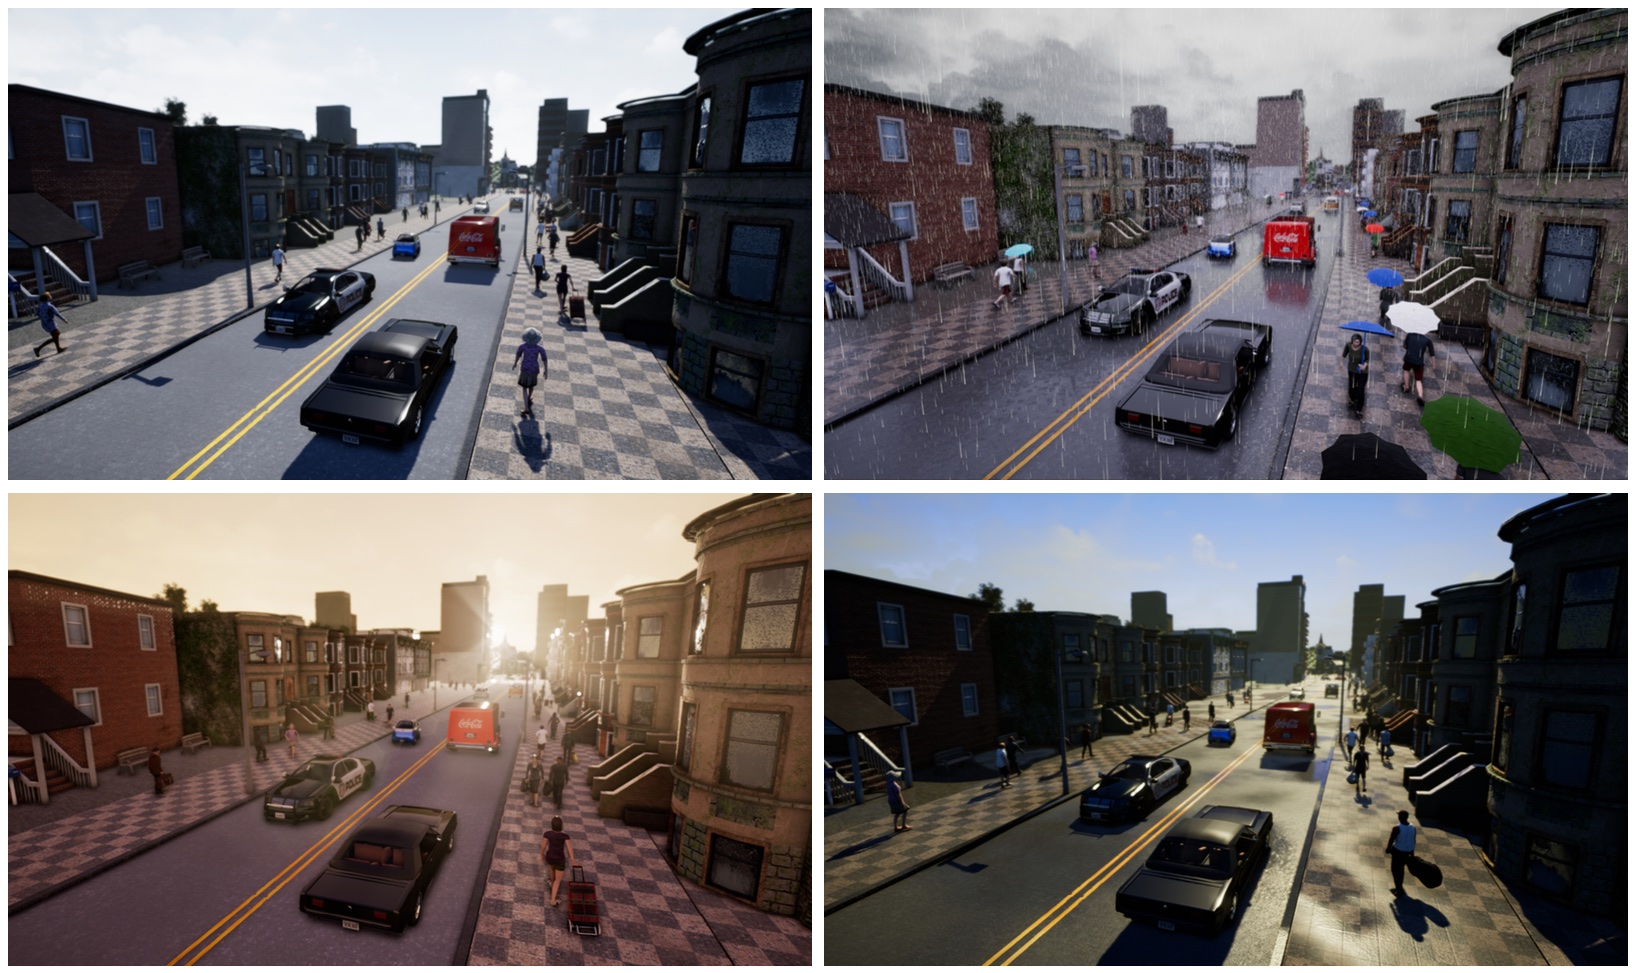
\includegraphics[width=.4\linewidth]{images/carlasim}
	\caption{CARLA Simulator}
	\label{fig:carlasim}
\end{figure}
CARLA merupakan simulator \textit{open source }untuk penelitian kendaraan otonom. CARLA telah dikembangkan untuk mendukung pengembangan pengoperasian, pelatihan, dan validasi sistem pengemudian otonom perkotaan. Dalam tambahan selain kode dan protokol \textit{open source}, CARLA menyediakan aset digital terbuka (tata letak perkotaan, bangunan, kendaraan) dan dapat digunakan secara bebas. Platform simulasi ini mendukung berbagai spesifikasi sensor yang fleksibel serta kondisi lingkungan yang beragam. \cite{cit:carlasim}

%------------------------------------------
\iffalse
\subsection{D4RL}
\begin{figure}[H] 
	\centering
	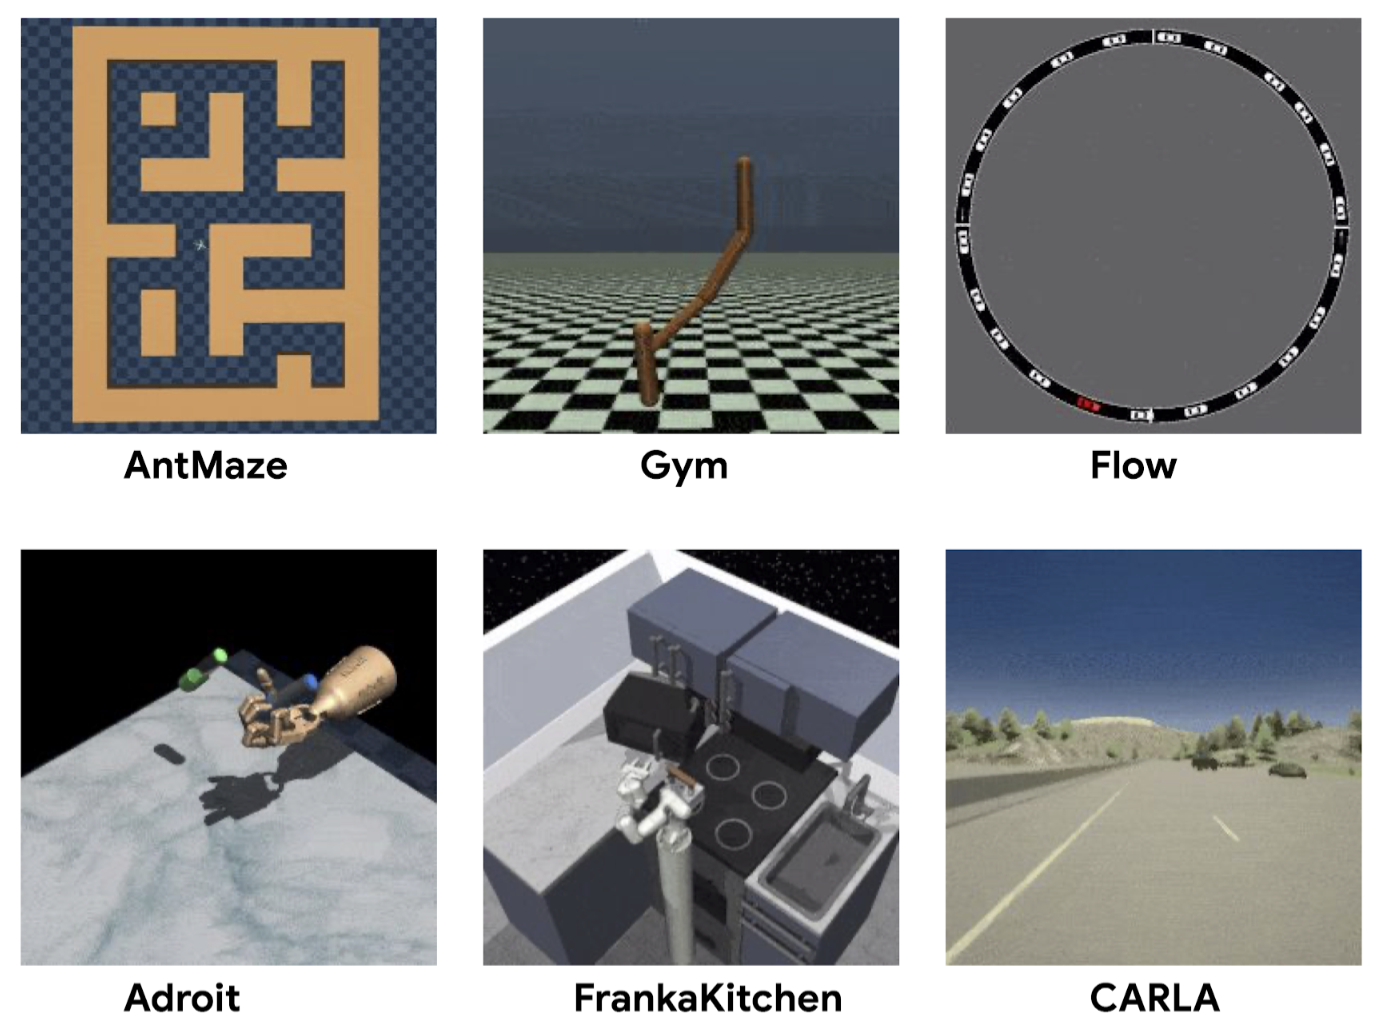
\includegraphics[width=.4\linewidth]{images/d4rl}
	\caption{D4RL: Datasets for Deep Data-Driven Reinforcement Learning \cite{cit:d4rl}}
	\label{fig:d4rl}
\end{figure}
D4RL atau \textit{Datasets for Deep Data-Driven Reinforcement Learning }adalah sebuah \textit{tool benchmark }yang dikhususkan untuk Offline Reinforcement Learning. Diberikan \textit{dataset }dan \textit{task }agar agen dapat melakukan berbagai \textit{task }yang seragam di lingkungan yang sama. \cite{cit:d4rl}
\fi
%------------------------------------------

\section{Penelitian Terkait}
\label{sec:penelitian_terkait}

Beberapa penelitian yang dapat ditemukan terkait dengan topik yang dibawakan oleh tugas akhir ini adalah:
\begin{enumerate}
	\item \textit{Driverless Car: Autonomous Driving Using Deep Reinforcement Learning in Urban Environment oleh A. R. Fayjie, S. Hossain, D. Oualid dan D. Lee (2018)}\newline
	Paper ini menyajikan \textit{deep reinforcement learning }untuk navigasi dan \textit{obstacle avoidance }dari mobil otonom, diaplikasikan dengan \textit{deep Q network }untuk mobil yang disimulasikan di daerah perkotaan. Menggunakan dua tipe sensor sebagai input, yaitu kamera dan laser di depan mobil tersebut. Simulasi yang digunakan diciptakan menggunakan Unity dan mensimulasikan daerah perkotaan dengan jalan 5 lajur.\cite{cit:1}
	
	\item \textit{Controlling an Autonomous Vehicle with Deep Reinforcement Learning oleh A. Folkers, M. Rick dan C. Büskens (2019)}\newline
	Paper ini menyajikan pendekatan kontrol untuk kendaraan otonom menggunakan \textit{deep reinforcement learning}. Melakukan penelitian untuk eksplorasi tempat parkir beserta \textit{obstacle avoidance }untuk kendaraan \textit{full-sized}. Penelitian tersebut merupakan salah satu penelitian pertama yang berhasil menerapkan \textit{deep reinforcement learning }pada kendaraan nyata.\cite{cit:2}
	
	\item \textit{Autonomous Driving in Roundabout Maneuvers Using Reinforcement Learning with Q-Learning}\newline
	Paper ini menyajikan manuver kendaraan otonom di bundaran dengan q-learning menggunakan simulator CARLA.\cite{cit:autonomdrive_roundabout_qlearning} Agent dalam paper tersebut mengambil data kamera rgb serta lidar sebagai parameter dari q-learning.
	
\end{enumerate}

\section{Gap Penelitian}
\label{sec:gap_penelitian}

Dari beberapa penelitian diatas, dapat dilihat ada \textit{gap} penelitian dimana paada penelitian yang dilakukan sebelumnya, belum ada yang melakukan riset mobil otonom untuk melakukan manuver pada bundaran atau u-turn menggunakan \textit{deep reinforcement learning}.
